\subsubsection{Tiny Code Generator}
\label{chap:QEMU_TCG}

QEMU's DBT takes the named of the Tiny Code Generator (TCG), and the basic 
code fragments it analyzes are called Translation Blocks (TB). These TBs are 
defined by jump instructions at machine code branch points and emulated hardware 
accesses (peripheral accesses) as boundaries\cite{QemuTCGOpsDevel} \cite{QemuTCGDirectBlockChaining}. 

The figure \ref{fig:TCG} illustrates the overall TCG architecture and workflow. Where the 
"Target Machine Code" corresponds to a TB, the blue part of the diagram represents 
the TCG, and the last block represent the "Host Machine Code".

\begin{figure}
    \centering
%    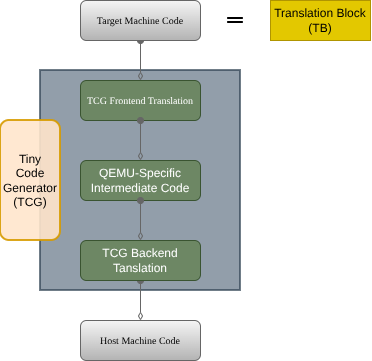
\includegraphics[width=0.5\textwidth]{Resources/Draw/TCG.png}
    \caption{Tiny Code Generator}
    \label{fig:TCG}
\end{figure}

As can be seen in \ref{fig:TCG}, the TCG operates through a two-phase translation 
process. In the first phase, the front-end translation part of the TCG, decodes 
the guest instructions into QEMU-specific intermediate representation (IR). 
Conceptually, this IR it is like an assembly language designed specifically for QEMU's 
compilation infrastructure. In the second phase, the back-end translation part of 
the TCG converts this intermediate representation into native host machine code, 
which is then directly executable on the host processor\cite{QemuTCGFrontendOps}\cite{QemuTCGBackendOps}.

The separation of front-end and back-end translation was due it provides 
significant advantages for QEMU's scalability. In order to support a new guest CPU 
architecture, developers need only implement a new front-end translator, while the 
back-end translation logic remains unchanged. Conversely, supporting QEMU on a 
new host architecture requires only back-end development, leaving guest architecture 
support unaffected. This modularity is the primary reason for QEMU's scalability 
across diverse hardware platforms and CPU architectures.